This chapter describes the previous work conducted at the University Stuttgart which delivers the essential components on which this thesis is build on.

\section{About the Design Changes Required for Enabling ECM Systems to Exploit Cloud Technology}
The main foundation for this thesis is the work from Shao~\cite{shao} which focused on the separation of monolithic Enterprise Content Management applications into isolated components. 
This split allows the separate ECM parts to be packaged and run within containers.
Until now ECM systems were usually deployed as large monolithic applications on private bare metal servers or virtual machines.
Since both of those approaches involve assumptions about the infrastructure which are not always true in cloud environments a new way of deployment is necessary.
\\
\\
First the applications are analyzed and decomposed based on their degree of coupling.
Tightly coupled components stay in the same container and loosely coupled components are split into separate containers.
Every container is composed with all essential dependencies and libraries to allow the operation as stand-alone service.
Further the shared data storage of monolithic ECM components is separated from the application logic so each component can use its own databases and file systems.
The cooperation between separated components happens over unified communication channels.
This split allows to exploit the potential of a cost effective scalability, continuous integration as well as continuous delivery.
\\
\\
The proof of concept which was developed during the thesis of Shao consists of an Enterprise Content Management system and a container platform.
As the ECM system the IBM Content Manager Enterprise Edition and as container virtualization technology Docker are selected.
The IBM system is chosen because of the historical relationship between the Institute of Parallel and Distributed Systems at the University Stuttgart and the IBM laboratories in B"oblingen.
Docker is selected since it is the most popular container virtualization technology with a large community and therefore many predefined images.
The ECM platform consists of four separate applications within Docker containers.
\textit{lsdbsrv} that contains the \textit{Data Catalog} and \textit{rmdbsrv} which incorporates the \textit{Object Catalog}.
Both containers are based on the public \textit{ibmcom/db2:latest} Docker image provided by IBM.
The other two components needed to be constructed manually based on the \textit{centos:7} image since there were no public Docker images available.
\textit{wasrm} contains the \textit{Resource Manager Application} as well as a HTTP server.
\textit{wasicn} includes the web client, the configuration database of the web client and a HTTP server.
The user interacts with the system through the web client which then sends or retrieves data from the \textit{Data Catalog}, \textit{Resource Manager} and \textit{Object Catalog}.
For the applications to be able to communicate with each other a virtual Docker network was created in the development environment.
~\cref{fig:gang_system} illustrates the resulting proof of concept with the separate components each inside its own container.
\begin{figure}[h]
    \centering
    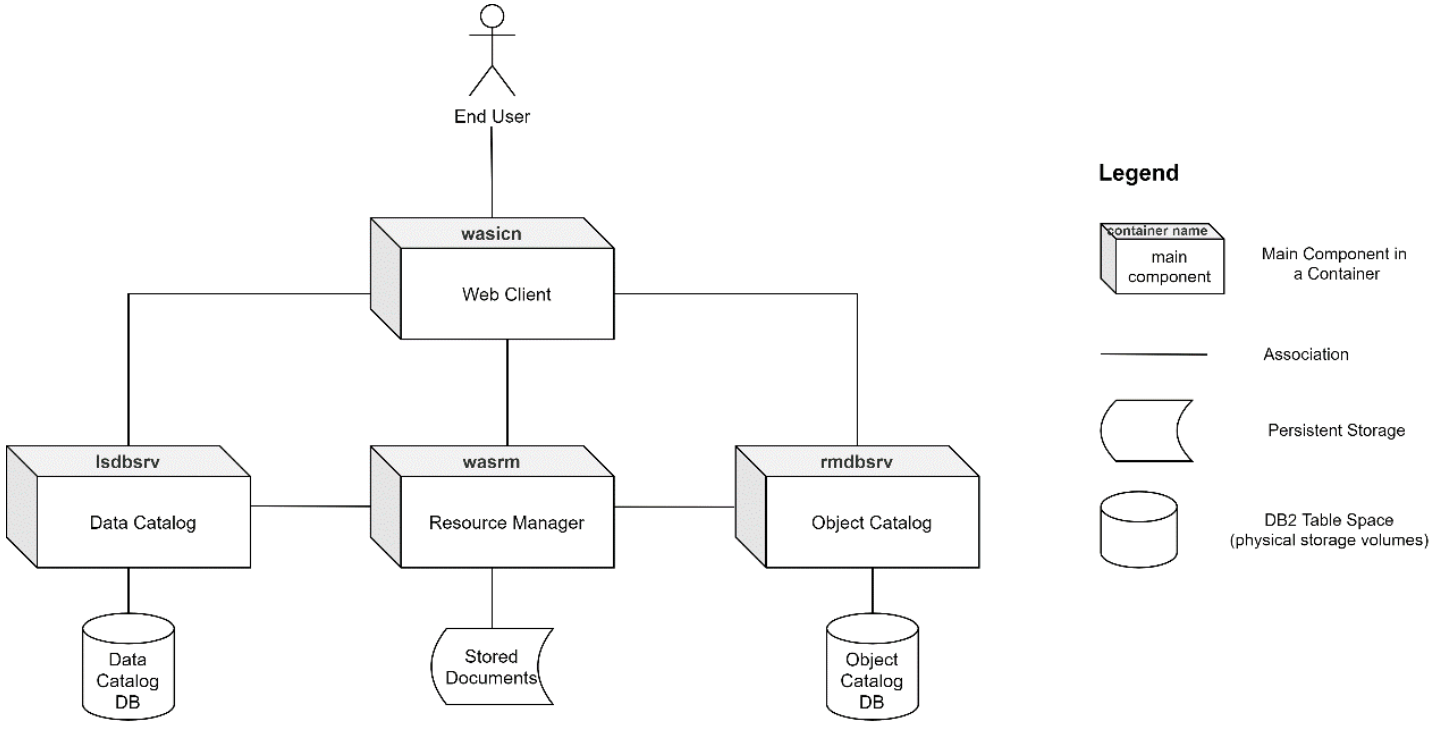
\includegraphics[width=\textwidth]{graphics/gang_system.png}
    \caption{Proof of Concept by Shao ~\cite{shao}}
    \label{fig:gang_system}
\end{figure}